% Created 2017-04-24 Mon 20:31
% Intended LaTeX compiler: pdflatex
\documentclass[sigconf]{acmart}
\usepackage[utf8]{inputenc}
\usepackage[T1]{fontenc}
\usepackage{graphicx}
\usepackage{grffile}
\usepackage{longtable}
\usepackage{wrapfig}
\usepackage{rotating}
\usepackage[normalem]{ulem}
\usepackage{amsmath}
\usepackage{textcomp}
\usepackage{amssymb}
\usepackage{capt-of}
\usepackage{hyperref}
\usepackage{epigraph}
\author{Nick Merrill, John Chuang}
\affiliation{%
  \institution{BioSENSE, UC Berkeley School of Information}
  \city{Berkeley} 
  \state{California, USA} 
}
\email{ffff@berkeley.edu}

\hypersetup{
 pdfauthor={},
 pdftitle={},
 pdfkeywords={},
 pdfsubject={},
 pdfcreator={Emacs 25.1.1 (Org mode 9.0.4)}, 
 pdflang={English}}

%% I do have one minor revisions I'd like to ask you to make. I found this sentence in the abstract a bit confusing: "I forward a theory of polemic computation, in which the feat of expending material (ecological, labor, and opportunity) costs, rather than particular computational results, exert agency in particular sociotechnical discourses."  Could you revise/clarify? In particular, I was confused by whether "costs" was acting as a noun or verb.

\begin{abstract}
In February of 2017, Google announced the  first SHA1 collision.
Using over nine quintillion computations (over 6,500 years of compute time),
a group of academic and industry researchers produced two different PDF files with identical SHA1 checksums.
But why? After all, SHA1 had already been deprecated by numerous standards and advisory bodies.
This paper uses the SHA1 collision compute as a site for surfacing the space of ecological risks, and sociotechnical rewards, associated with the performance of large computes.
I forward a theory of polemic computation,
in which computes
exert agency in sociotechnical discourses
not through computational results,
but through \textit{feats},
the expenditure of significant material resources.
This paper does not make specific claims about the (ecological, political, labor) limits within which polemic computes must operate in order to be considered acceptable.
Instead, this paper raises the question of how such limits could be established, in the face of polemic computes' significant costs and difficult-to-measure rewards.
\end{abstract}


\begin{CCSXML}
<ccs2012>
<concept>
<concept_id>10010405.10010476</concept_id>
<concept_desc>Applied computing~Computers in other domains</concept_desc>
<concept_significance>500</concept_significance>
</concept>
<concept>
<concept_id>10003120.10003121.10003126</concept_id>
<concept_desc>Human-centered computing~HCI theory, concepts and models</concept_desc>
<concept_significance>300</concept_significance>
</concept>
</ccs2012>
\end{CCSXML}

\ccsdesc[500]{Applied computing~Computers in other domains}
\ccsdesc[300]{Human-centered computing~HCI theory, concepts and models}

% We no longer use \terms command
%\terms{Theory}

\keywords{theory, limits, polemics, charisma}

\copyrightyear{2017}
\acmYear{2017}
\setcopyright{acmlicensed}
\acmConference{LIMITS '17}{June 22-24, 2017}{Santa Barbara, CA, USA}\acmPrice{15.00}\acmDOI{http://dx.doi.org/10.1145/3080556.3084082}
\acmISBN{978-1-4503-4950-5/17/06}
\usepackage[T1]{fontenc}
\usepackage{lmodern}
\date{\today}
\title{Better Not to Know?\\\medskip
\large The SHA1 Collision \& the Limits of Polemic Computation}
\hypersetup{
 pdfauthor={},
 pdftitle={Better Not to Know?},
 pdfkeywords={},
 pdfsubject={},
 pdfcreator={Emacs 25.1.1 (Org mode 9.0.4)}, 
 pdflang={English}}
\begin{document}

\maketitle

\epigraph{I insist on the fact that there is generally no growth but only a luxurious squandering of energy in every form!}{Georges Batailles, \textit{The Accursed Share}}


\section{Introduction}
\label{sec:org75eddc9}

From protein folding to the discovery of novel drugs,
large computes can discover valuable answers to important questions
\cite{Anderson2004}.
They also invariably enter into sociotechnical discourses,
taking active agency in the politics, economics and epistemologies 
of particular fields, disciplines and institutions \cite{Ames2015}.
Indeed, computes are material artifacts, manifest in space and time,
and share an essential form of material agency with all things \cite{Bennett2013a,Winner2003}.

This paper reads the SHA1 collision compute (Sections 2 and 3), 
and the various sociotechnical entanglements that motivated its performance (Section 4).
in order to motivate and explain a theory of \emph{polemic computation} (Section 5).
Polemic computations, I claim, enter into sociotechnical discourses through the \emph{feat} of their completion, rather than by virtue of a particular result computed.
In the case of the SHA1 collision, the compute as a feat compute entered into existing discourses of authenticity, privacy and security on the Internet (Section 4).

The performance of the SHA1 collison weighed political goals around cybersecurity against fiscal, ecological, and opportunity costs.
This paper does not opine on whether its performance was ``right'' or ``wrong,'' acceptable or not, justified or unjustified.
Rather, it aims to raise discussion around the limits within which polemic computes can be considered acceptable (Section 6).
When are feats are justified? 
When should feats be resisted, due to their costs? 
Through what moral, ethical, econometric frameworks could such questions even be evaluated? 
In these questions lurk the shadows of larger debates around how, and why computations are deemed acceptable (and for whom).
How do designations of acceptability relate to the costs fo computes, and to the social structures that are strengthened, weakened, or reified by their performance?

\section{Background}
\label{sec:org79d5f75}


Before discussing Google's large compute in depth,
this section gives some background on SHA1, and cryptographic hash functions in general.
Cryptographic hash functions are ``one way'' functions: 
they take some data, and produce some new data, such that the original data cannot be recovered from the new data. The output of the hash function is simply called a \emph{hash}.

SHA1 is one cryptographic hash function, designed by the NSA in the early 1990s.
The hashes output by SHA1 are typically 40 digits, regardless of the size of the input data.
It is used in many version control applications to refer uniquely to files, 
or to check for corrupted files. 
Crucially, as I will discuss in Section 3, SHA1 is also used in security-oriented protocols such as SSH/TLS.


\subsection{SHA1 collisions}
\label{sec:org67ccb05}

Hashes should relate uniquely to input data: 
two different inputs should never produce the same hash (even though hashes are much smaller than the original data).
A \emph{collision} refers to the breakdown of this property,
in which two different input data produce identical hashes.

Collisions break several common uses of SHA1. 
Amusingly, a test in the WebKit browser engine's source code
broke the version control system used for that repository \cite{Koivisto2017}.
Subversion, on which WebKit's repository relies, uses SHA-1 hashes to refer uniquely to source code files.
A test aimed at capturing the SHA-1 collision incidentally included two different files with the same hash, 
breaking the version control software and temporarily halting development.
(Git sidesteps this issue by using an additional code  attached to the SHA-1 hash \cite{Torvalds2017}).

In the case of SSL/TLS, the protocol for encrypted and authenticated communication on the web, SHA1 collisions could have even more severe consequences;
namely, breaks to authenticity and/or security in web connections.
Section 5 will return to TLS vulnerability in more detail.

\subsection{SHA1 collisions in theory}
\label{sec:org2c6f7c5}

In discussing the safey of particular hash functions, two questions must be asked:
(1) how long would it take to find a collision by brute force?, and 
(2) is there any algorithm that allows us to find a collision faster than the brute force method?
For the brute force method, the odds of finding a SHA1 collision by chance are one/2\(^{\text{80}}\)
\cite{Schneier2005}.
In general, the security of this brute-force attack is judged relative to the outer edge of high-end hardware, and hash functions are expected to be retired in time, as computers grow more powerful.
However, this 2\(^{\text{80}}\) space of possibilities in the search for a collision is not considered feasible, so SHA1 appears safe.

In 2005, however, Wang, Yin \& Yu found an algorithm to produce SHA1 collisions in under 2\(^{\text{69}}\) calculations (about 2,0000 times faster than brute force)
\cite{Wang2005}.
(Other work had suggested possible weaknesses of SHA1 earlier \cite{Biham2005}).
While such a compute was, at the time, considered outside the limits of even powerful adversaries,
the result caused concern among cryptographers \cite{Schneier2005}.
By 2011, a 2\(^{\text{61}}\)-calculation attack was discovered \cite{Stevens2013a},
and by the mid 2010s, the developers of most major browsers had announced plans to stop accepting SHA1 SSL certificates 
\cite{Mozilla2017,Sleevi2014}.

\section{Performing a Collision}
\label{sec:org307f820}

The study in question here produced two PDFs with different content, but identical SHA1 hashes.
\cite{Stevens2017}.
The authors released the source code for performing the attack
\cite{Stevens2017github}.

This feat required 2\(^{\text{63.1}}\) computations. 
Compared to the 2\(^{\text{61}}\) theoretical attack, the practical attack took a bit longer due to the communication overhead required to coordinate computations across several datacenters, and due to the relative inefficiency of using GPUs rather than CPUs.

In practice, the computation that produced the SHA1 collision required 6,500 years of CPU time and 110 years of GPU time. While this number certainly sounds high, with 600,000 cores, each running two threads, it could require only a few days of compute time.

Of course, time is not the only cost to consider.
Computation is material, physically instantiated, and has ecological consequences.
Beyond monetary cost, such large computations carry very real costs in energy.
Since the implementation details of the infrastructures used for the large collision compute are not entirely knowable from the paper,
it is difficult to estimate this energy cost, but, as a rough point of comparson,
the monetary cost of such a compute on Cray supercomputers would be on the order of one million USD 
(though such estimates might vary widely in either direction from system to system)
\cite{Pautsch2016}.
In any case, such a figure is a tiny sliver of Alphabet Inc.'s 90 billion USD revenue as of 2016.

This section gave background on SHA1 collisions, 
and gave context for the costs (in time and energy) of the SHA1 collision compute.
The following section details possible explanations for why the computation was performed
in practice, rather than simply discussed in theory.

\section{Explaining why the compute happened}
\label{sec:org8536c9d}

\begin{figure*}
\centering
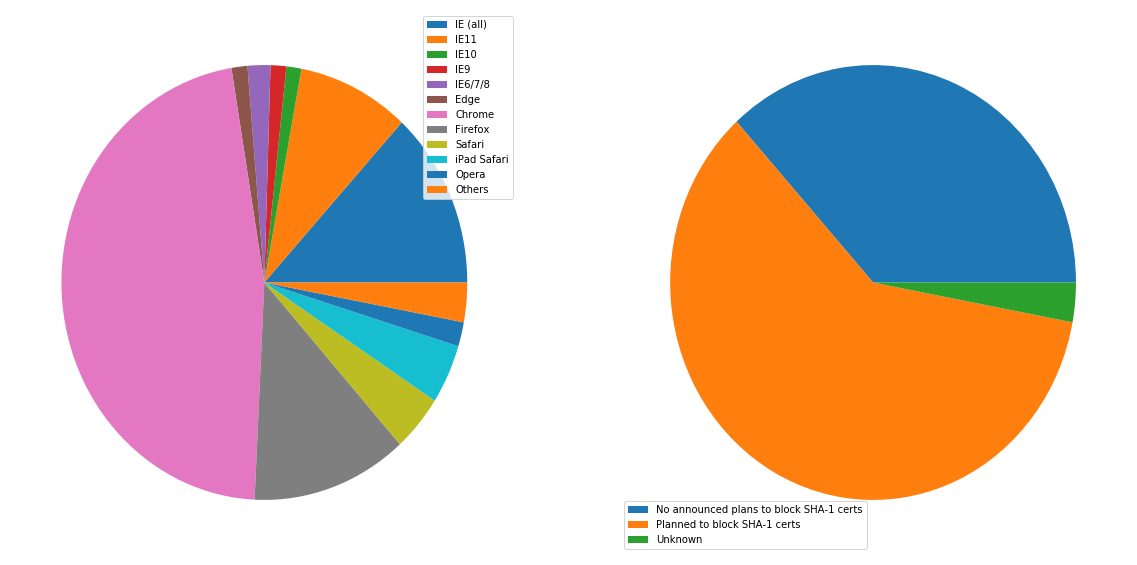
\includegraphics[width=.9\linewidth]{./figures/browser-share.png}
\caption{Proportion of Internet users by browser (left), and proportion of browser usage with plans to block SHA-1 certificates (right). A majority of browsers had already announced plans to deprecate SHA-1 certificates, even before the collision was demonstrated. However, some older browsers have continued to accept these certificates.}
\end{figure*}

Since a theoretical result already existed showing a SHA1 collision was possible, 
one might rightly wonder why researchers would go through a great deal of time and effort
(not to mention a great deal of expense, both monetary and ecological)
to produce artifacts of no practical purpose (different PDFs with identical checksums).
What are the possible benefits?

In this section I argue that
the SHA1 collision compute had essentially polemic goals.
It was performed not to know a particular answer
(as the PDFs themselves are not useful as artifacts), 
but to know that such an answer \emph{has} been found,
as opposed to \emph{can} be found.
I argue that the performance of this collision compute
was necessarily entangled in a particular sociotechnical discourse,
and aimed to change opinions and behavior among specific groups of stakeholders.
This section focuses in particular on those involved in the ecosystem of SSL certificates: browsers, webmasters, and the certificate authorities (CAs) tasked with generating certificates.

\subsection{Practice versus theory}
\label{sec:orga900aec}

Before progressing onto a discussion of this compute on the ecosystem of SSL certificates,
we must briefly argue for why an argument of academic interest does not sufficiently explain why this compute was performed, rather than simply discussed.

The computation here ended up being more difficult than theoretical results indicated due to the storage and communication requirements necessary to perform the work across multiple datacenters. 
The collision compute reveals details relevant
to knowing how realistic the threat is in practice. 
Of course, given that SHA1 has already been widely deprecated, this explanation does not in itself answer why such an exercise was considered necessary.
After all, one would not need to know the cost in practice of such an exercise without some reason.

Indeed, one reason, aside from the particular answer computed, is that the compute raises a question and challenge to users of SHA1:
``Do SHA1 users have assets worth at least as much as the cost of this compute?''
All cryptography can be broken with sufficient computational time.
This result shows that a powerful attack (such as Google) can indeed break SHA1 with some knowable resources.
And, surely, if Google can perform such an attack, a government actor could do so as well.

Of course, some users of SHA1 did not care much about the demonstrated attack.
Linus Torvalds, developer of the Git version control software (which relies on SHA1 to refer to files), reported no immediate concern.
``Do we want to migrate to another hash? Yes. Is it 'game over' for SHA1 like people want to say? Probably not.'' \cite{Torvalds2017}.
The following section explains the performance of this collision in the context of 
an application in which stakes are potentially much higher:
the issuance of SSL certificates, some of which rely on SHA1 to provide cryptographic guarantees.

\subsection{SHA1 and SSL Certificates}
\label{sec:org249a350}

\begin{figure}[t!]
\centering
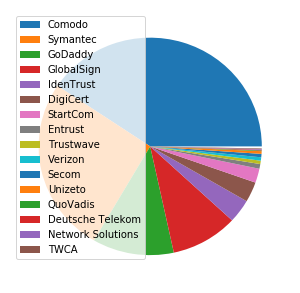
\includegraphics[width=.9\linewidth]{./figures/ca-share.png}
\caption{The distribution of SSL certificates on the web, by certificate authority (CA). While a few CAs lead in market share, a large number of smaller CAs issue a smaller proportion of certificates. Compared to the relatively more centralized market of browser share (Figure 1), this market fragmentation makes enforcement more difficult, as coordination and consensus must be achieved over a larger number of stakeholders.}
\end{figure}

SHA1 is also used in the issuance of (especially older) SSL certificates.
(SSL certificates
provide a token of the authenticity of a user's connection to a webpage,
and encrypts data end-to-end).
This practical result showed that someone with the power to perform a SHA1 collision could
now make a fake certificate for a website with that uses SHA1 for its TLS.
Such a false certificate could
be used to convince a victim that they are communicating with a given website,
when in fact they are communicating with the attacker.

SSL certificates are issued by Certificate Authorities (CAs), which in theory abide by 
regulations set by the CA/Browser Forum, a standards-setting body.
Here unravels a more complex story of regulation and standards bodies,
as well as stakeholders for whom a change away from SHA1 could incur significant monetary costs.
The following sections examine the polemic impact of this attack on both CAs, and browser developers. 

\subsubsection{Certificate authorities}
\label{sec:org205f4ac}

First, the SHA1 attack can be mediated entirely by
replacing old SHA1 certificates with newer ones using SHA-2 or SHA-3.
Second, CAs that abide by CA/Browser Forum rules are already forbidden from issuing SHA1 certificates. (They are additionally required to insert at least 64 bits of randomness, in an effort to mitigate devastating effects from future cryptographic breaks) \cite{Stevens2017}.

However, Since CAs are decentralized, and since SSL issues (website administrators) do not routinely check issued SSL certificates for these properties, enforcing these regulations is a perennial challenge for the CA/Browser Forum. It is not clear that CAs were abiding by either of these rules.
There exists a long tail of small certificate authorities (Figure 1), in comparison to the relative centralization of browser production (Figure 2) \cite{Q-Success2017}.
Assuming they were not, one explanation for performing this compute is that doing so would encourage CAs (and webmasters) to take more seriously the threat posed by SHA1,
putting some real pressure on them by freely releasing code that could result in forged certificates \cite{Stevens2017github}.

In effect, the very existence of an exploit makes CAs who continue not to abide by CA/F rules more liable.
Thus, this rather costly collision compute worked to an extent as an agent of enforcement,
``correcting'' (that is, enforcing a perspective upon) CAs in ways existing standards bodies were unable to do.


\subsubsection{Browser developers}
\label{sec:orgae7ef28}

Alongside the issue of enforcing proper security practices on a decentralized system of certificate authorities, 
a separate ecosystem of browser developers exercises independent authority to accept, or reject, certificates issued by CAs.
While browser production is also decentralized, it is less so than CAs (Figure 2)
\cite{Buckler2016}.

According to these statistics, the majority of browsers on the web had already agreed to stop accepting SHA1 SSL certificates,
even before this compute took place
\cite{Sleevi2014,Mozilla2017}.
So, regardless of what certificate authorities do, users of these browsers would have been protected from any vulnerabilities in SHA1, 
and the CAs would have faced additional market pressure to move away from SHA1.

If the performance of the collision compute was not necessary to change behaviors among browser developers
(and thus to protect users),
why was it performed?
One explanation may come from the press room.
Browser developers such as Mozilla and Google have received criticism for their decision to reject SHA1 certificates, even from other industry leaders such as Facebook \cite{Stamos2015}, given the still-theoretical nature of the hash's vulnerability
Thus, another dimension of this compute's polemic aims
relates to browser PR, undercutting claims that the decision to deprecate SHA1 was premature.
Crucially, browsers has a vested interest in security:
browsers need their users to feel secure, as customers will flee if they do not feel safe shopping and communicating on the Internet.

\section{The polemics of actually doing}
\label{sec:orgb1d5a42}

The prior section gave sociotechnical context for the performance of the SHA1 collision compute,
giving many explanations across a wide variety of contexts.
However, as of now, we lack a theory for systematically typifying these disparate explanations.
In this section, I propose a definition of \emph{polemic computation} to describe motivations for performing computes such as those above (Section 5.1).
Namely, we propose that some computation is performed because there is a polemic power to doing so, 
and that the material resources expended on such a computation take agency in particular sociotechnical debates.
We tie this theory to that of charismatic technology (Section 5.2)
and to critical design (Section 5.3)
in centering the material nature of performed computation
in describing its agential power in sociotechnical discourses.

\subsection{Defining polemic computation}
\label{sec:org781cf9a}

This paper defines \emph{polemic computation} 
as a computation enacted (rather than discussed)
in order to forward an argument or ideology.
Crucially, computations are material artifacts, 
produced in time and energy 
\cite{Dourish2011a}.
Their performance or enactment also requires 
specialized technical expertise in the form of labor.
Polemic computes are at once feats and artifacts, which act \cite{Ames2015} 
in sociotechnical debates.
The following sections relate this theory of polemic computations
to other theories of charismatic technology and critical design,
highlighting the relevant differences to our theories.

\subsection{Charismatic technology}
\label{sec:org1805277}

Polemic computation can be said to ``work'' in part 
because it is animated by ideological frameworks.
In the case of the SHA1 computation,
ideals that web communications \emph{should} be private and authenticated
very much animate the particular computations that occurred.
These ideals become especially clear when one examines the motivations for actually performing the compute,
even though they were already discussed in theory.

In this way, polemic computation draws strongly from Ames' theory of \emph{charismatic technology}
\cite{Ames2015}.
Drawing on actor-network theory, charismatic technology would ascribe the very artifact of the computation
(a material artifact produced by material means \cite{Dourish2011a,Bennett2013a})
agency in the technosocial discourses around privacy and security.
Much like in Ames case of the One Laptop Per Child project,
polemic computation aims to change behavior and beliefs among specific stakeholders in specific debates.

As with charisma,
power is central to polemic computing.
Here, power plays in through the resources required to perform the compute.
However, in contrast to charismatic technology, polemic computation 
centers the material act of computing as a \emph{feat} with costs in time and energy.
In energy, computation expends valuable and scarce ecological resources \cite{SixSilberman2015}.
In time and energy, computational incurs opportunity costs, through answers that could have been computed but were not.

Rather than computing answers, polemic computation uses the material feat of expenditure 
to work as an agent in technosocial discourse.
Indeed, the SHA1 collision demonstrated an attack feasible only for highly resourceful actors (for now). 
Such actors might be a government or, apparently, Google.
Thus, this collision demonstrated not only the considerable resources required to exploit SHA1,
but the vast resources that Google must have, if it is able to spend so heavily on a project with essentially polemic aims.

\subsection{Critical design}
\label{sec:org81f7ca4}

Another strand of research that explicitly centers the agency of technological artifacts
is critical design \cite{Dunne2001}.
Critical design seeks to harness the agency of technical artifacts 
to challenge assumptions or surface lurking cultural narratives.
In many ways, polemic computation serves as a critical artifact.
The SHA1 collision compute, for example, 
called out the poor security practices of many certificate authorities.
Specifically, the material production of the computation,
combined with its almost satirical nature (the compute produced PDFs),
acted to \emph{define} what is and is not a poor security practice for certificate authorities.
Much in the tradition of critical design
used its material power \cite{Bennett2013a} along with a touch of humor, to enter into technosocial debates and imaginaries.

\section{When is it better not to know?}
\label{sec:orgffe5e6d}

So far, this paper described the SHA1 compute, situating it relative to particular strategic, political goals in cybersecurity (goals in which Google holds a large economic investment, as a distributor of web browser and Internet services).
I used this case to motivate a theory of \emph{polemic computation}, which captures the ``feat''-like nature of this compute, as a way of describing the agency that this compute had within the sociotechnical discourse it sought to enter.

The fiscal, ecological, and opportunity costs associated with the SHA-1 compute must have been weighed against these political goals. Future work could attempt to ask those involved first-hand with the work how such costs were considered.
However, this paper is not primarily concerned with whether or not the performance of the SHA-1 compute was justified. 
Instead, the major outstanding question for this paper surrounds how we could reasonably consider questions about when polemic computations are (or are not) justified.

Within what limits are polemic computations acceptable?
When, how, and for whom are those limits justified? 
When (and how) should ``feats'' be resisted, because the resources they consume could be put to other endeavors? 
This section discusses how such questions might be answered, raising challenges for future work. 
I discuss the generalizability of this theory before concluding.

\subsection{Frameworks for evaluation}
\label{sec:org5e2877f}
Above, we raise the question of how we might evaluate whether a polemic computations is acceptable or not.
Through what frameworks could such questions be evaluated? 
On one hand, the ecological impact of particular computes weighs heavily as a tangible cost to performing computes.
One might also discuss opportunity costs with regard to what else could be computed.
Both of these modes of evaluation beg econometric methods of analysis, 
operationalizing costs as expenditures in energy, resources, labor, capital.

However, these economic costs must be weighed against polemic goals, which do not lend themselves as straightforwardly to the same analyses.
How can we evaluate the ``worth'' of the polemic goals of these computes?
Moral and ethical frameworks could evaluate the sociotechnical aims forwarded by particular computes. 
Future work should more closely examine how such guidelines might be constructed, such that they stand a chance at enabling evaluation against material costs.
After all, it is not immediately clear what sorts of ethical, regulatory or legal frameworks 
might serve to create bounding conditions, outside of which certain computes are deemed unacceptable.
What is clear, however, is that these frameworks (and econometric ones) will inevitably
embed particular politics and worldviews as they come construct designations of acceptability.

Finally, even if such frameworks for evaluating computes existed, it is not immediately clear how they could be used to our benefit. 
Would legal or regulatory frameworks be most appropriate?
Or social pressure among technical practitioners?
Future work could examine these questions more closely,
and in the context of different types of computes, or different moral and ethical frameworks.


\subsection{Generalizing polemic computation}
\label{sec:org97fdca4}
Finally, this work raises the question of how general this theory of polemic computation must be.
Do any computes exist that are not, in some way, polemic?
In other words, are there any computations for which the ``feat'' of having performed computation do \textbf{not} itself work as an actor in technosocial discourses?
After all, computes are everywhere, and increasingly so in an era of connected devices in the home, workplace, and on the body. 
What is the energy, labor, time of the computes these devices perform ``worth,'' relative to other things that could be done?
With many IoT applications (like ''smart stockrooms'' or even ''smart cities,'') this question begs an econometric answer.
But, what about the polemic sides of these computes: the sense in which these computes are not just the producers of answers, but feats, which serve to reinforce, reify, or introduce particular politics, systems of commerce, oppress liberation?

Future work could probe this question more deeply.
Fruitful cases for further study might include the search for novel drugs (which is inexorably tied in the particular economics of the pharmaceutical industry), or cryptocurrencies such as Bitcoin (which use difficult computations to produce notions of economic value).
By examining these different cases, we might refine our tools for evaluating polemic dimensions to computes more generally.
In so doing, we may begin to make headway on the difficult questions raised in this section, around how computes can be considered acceptable with regard to particular goals.

\section{Conclusion}
\label{sec:org0bfe483}

As computation grows in its ubiquity as a material substrate of contemporary life in the developed world,
we will only have more things to compute,
and more things to compute them with.
Using the example of a particular large-scale compute,
this paper highlights broader tensions about when and when not to compute.
How can we select what we expend our increasingly precious resources on?
Indeed, how do we decide which computes are considered acceptable, and what goes into such decisions?
Clarifying our answers to these questions will prove critical in our more resource-constrained future.

\section{Acknowledgements}
\label{sec:org7088584}
Many thanks to Donald Patterson, Ellen Zegura, Morgan Aimes, Nick Doty, Anette Greiner, Sebastian Benthall and John Chuang for their comments and conversations. 
This work was supported by a grant from the UC Berkeley Center for Long-Term Cybersecurity (CLTC).


\bibliographystyle{ACM-Reference-Format}
\bibliography{refs}
\end{document}
